% Loki docker plugin causes all the containers to be unable to restart or kill. The alternative is to use the
% json-file driver with custom options. The json-file driver is the default driver for Docker.
% https://stackoverflow.com/questions/38567355/docker-compose-global-level-logging
% https://howchoo.com/devops/how-to-add-a-health-check-to-your-docker-container

\sect{Docker}{docker}
Docker es una plataforma software que permite el desarrollo, despliegue y ejecución de aplicaciones de forma rápida y
cómoda, separando la aplicación de la infraestructura, permitiendo ejecutar múltiples aplicaciones en un mismo servidor
(ver figura~\ref{fig:docker-container-infrastructure}).\ Esto se realiza empaquetando la
aplicación, sus dependencias y otras herramientas necesarias para su ejecución en lo que se denominan
\boldFont{contenedores}, que son instancias ejecutables de una imagen de Docker.\ Las \boldFont{imágenes} son
ficheros de solo lectura que contienen las instrucciones necesarias para crear un contenedor, y normalmente se basan
en otras imágenes añadiendo o modificando configuraciones~\cite{docker-docs}.

\begin{figure}[ht]
	\centering
	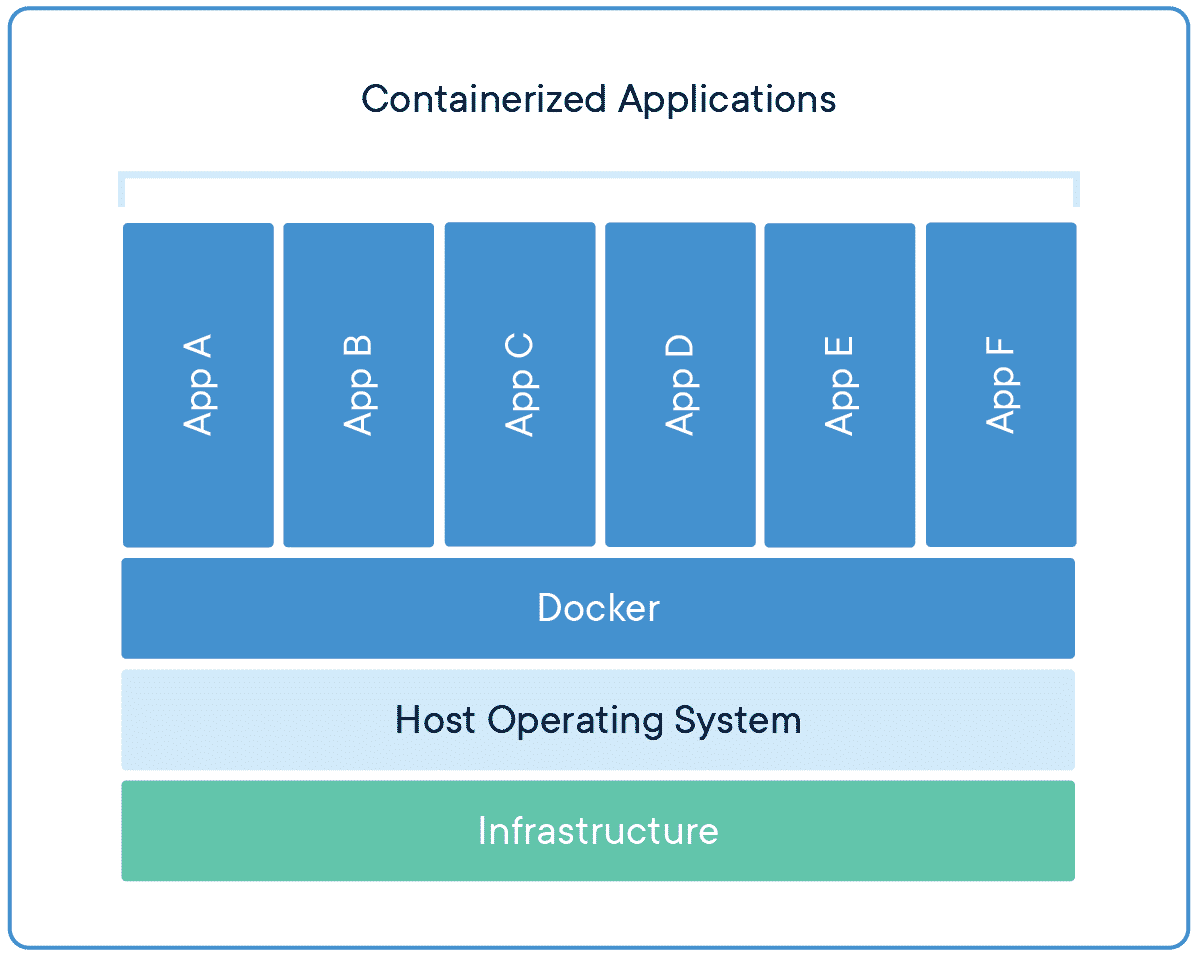
\includegraphics[width=0.8\textwidth]{res/images/container-what-is-container}
	\caption{Infrastructura docker. Fuente: \url{https://www.docker.com/resources/what-container}.}
	\label{fig:docker-container-infrastructure}
\end{figure}

En el desarrollo de la aplicación se ha utilizado Docker para la creación de una imagen que contenga todo el código de
la aplicación, así como las variables de entorno necesarias para su correcto funcionamiento.\ Se ha
utilizado la herramienta \monoFont{docker-compose}, que permite definir y ejecutar contenedores Docker de manera
sencilla.\ Para la configuración de los contenedores se dispone del fichero \monoFont{docker-compose.yaml}, que se
encuentra en la raíz del proyecto y define los servicios que se ejecutarán en los contenedores, así como
las dependencias entre ellos.

Debido a que cada vez que se elimina un contenedor (al reiniciar el sistema o al generar de nuevo la imagen de la
aplicación para incluir cambios del código) se pierden los datos, la \boldFont{persistencia} de los mismos y de sus
configuraciones es \boldFont{necesaria}.\ Para lograr esto, se usan \boldFont{volúmenes}, que son directorios creados y
gestionados por Docker que se almacenan en el sistema de archivos del host, y que se montan en los contenedores cuando
se inicializan~\cite{docker-volumes}.\ De esta forma, los datos no se pierden al eliminar el contenedor.\ Los
volúmenes se definen en el mismo fichero \monoFont{docker-compose.yaml} mediante la opción \monoFont{volumes} y son
los siguientes:

\begin{itemize}
	\item \monoFont{rschat-db}: contiene los datos y script inicial de la base de datos.
	\item \monoFont{rschat-logs}: contiene los ficheros de registro de la aplicación.
	\item \monoFont{grafana-storage}: contiene la configuración de Grafana.
\end{itemize}

\begin{figure}[ht]
	\centering
	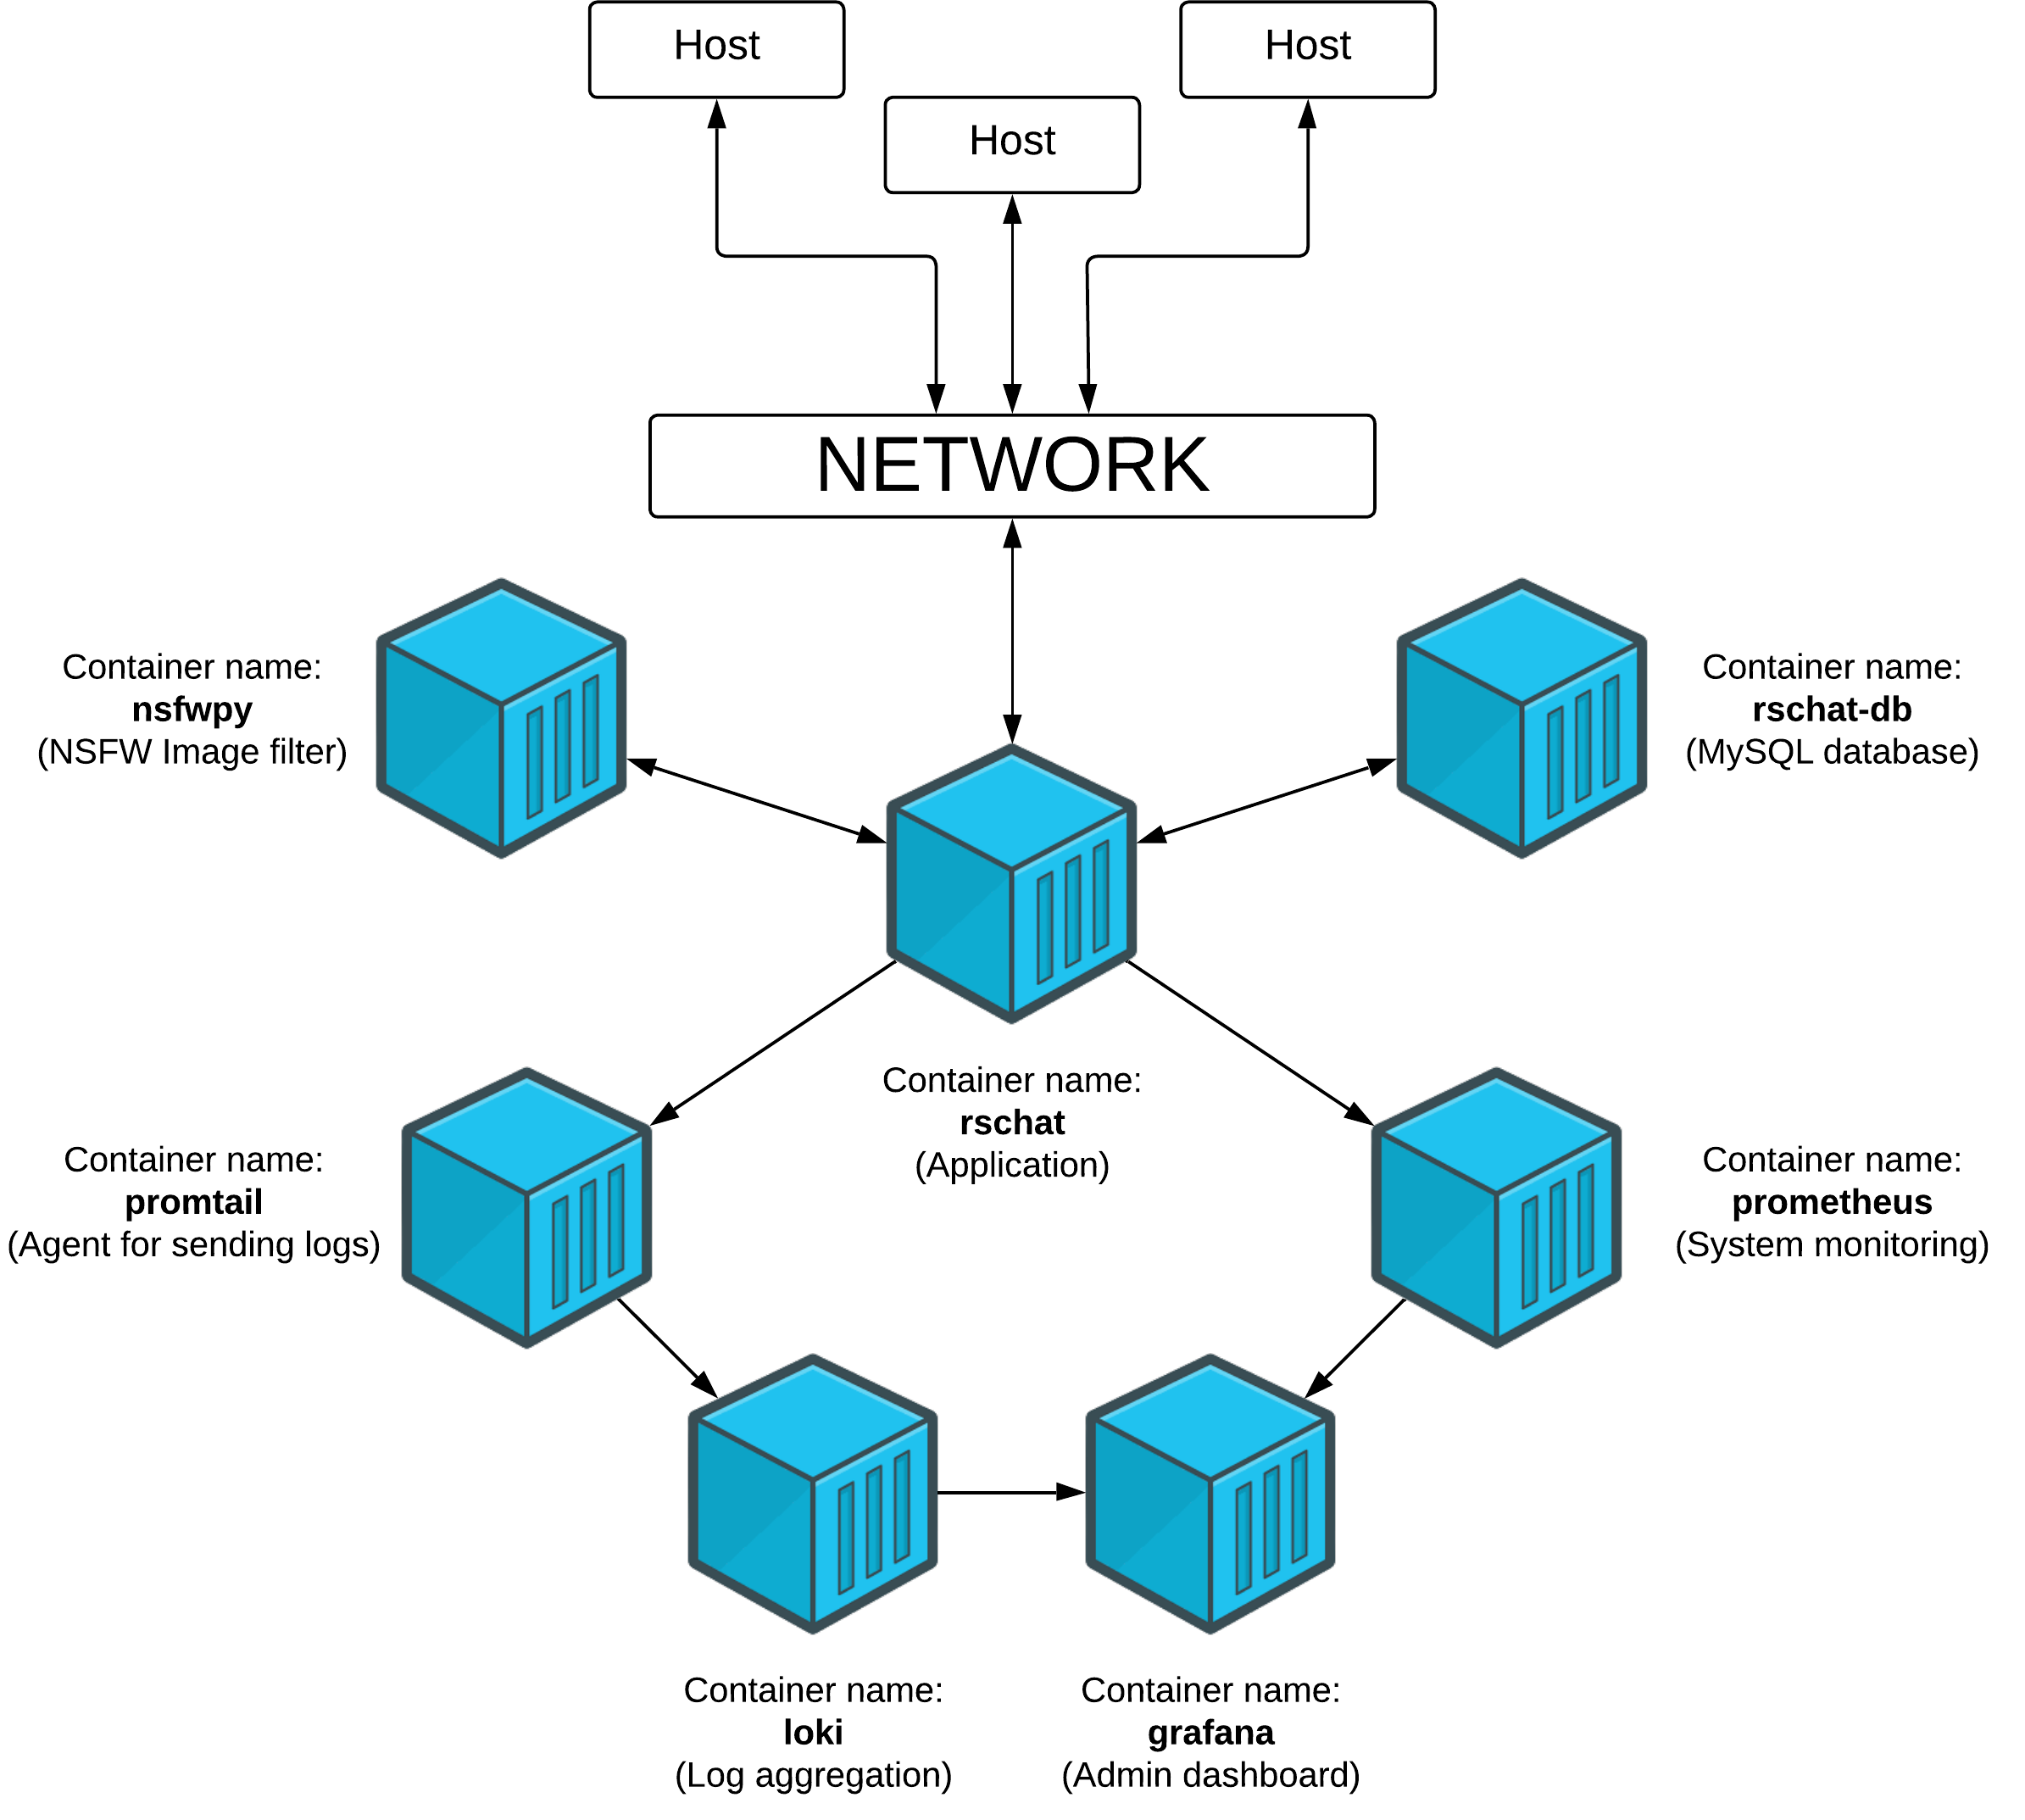
\includegraphics[width=0.8\textwidth]{res/images/InfraestructuraDockerRSChat}
	\caption{Diagrama de relación entre los contenedores Docker utilizados en RS Chat.}
	\label{fig:docker-container-diagram}
\end{figure}

A continuación, se mencionan todos los contenedores utilizados para la aplicación junto con una breve descripción de
cada uno de ellos.

	{\footnotesize Nota: los nombres marcados con el símbolo \textsuperscript{\textasteriskcentered} se describirán en
detalle más adelante.}

\begin{itemize}
	\item \monoFont{rschat}: Contenedor que ejecuta el backend de la aplicación.
	\item \monoFont{rschat-db}: Contenedor que ejecuta la base de datos MySQL\@.
	\item \monoFont{prometheus\textsuperscript{\textasteriskcentered}}: Contenedor que ejecuta el servidor de métricas
	de Prometheus.
	\item \monoFont{grafana\textsuperscript{\textasteriskcentered}}: Contenedor que ejecuta el panel de observabilidad
	de Grafana.
	\item \monoFont{loki\textsuperscript{\textasteriskcentered}}: Contenedor que ejecuta el servidor de logs Loki.
	\item \monoFont{promtail\textsuperscript{\textasteriskcentered}}: Contenedor que ejecuta el agente de logs
	Promtail.
	\item \monoFont{nsfwpy\textsuperscript{\textasteriskcentered}}: Contenedor que ejecuta el servicio de detección de
	contenidos inapropiados\@.
\end{itemize}
\label{itm:docker-compose-services}

\subsect{Prometheus (Métricas)}{prometheus}
Prometheus es un conjunto de herramientas de código abierto para la \boldFont{monitorización} de sistemas y
\boldFont{alertas}, que recoge y
almacena las métricas con la marca de tiempo cuando se producen, incluyendo etiquetas (clave-valor) de manera
opcional~\cite{prometheus-overview}.
Estas métricas se utilizan para determinar el funcionamiento y estado de la aplicación en tiempo real, permitiendo
diagnosticar problemas de rendimiento o recursos de una manera rápida y sencilla.\ Para habilitar la exportación de
las métricas (de manera automática) por parte de la aplicación, hay que realizar las siguientes cambios en los
ficheros de configuración:

\begin{itemize}
	\item Añadir 2 librerías en el fichero \monoFont{pom.xml}~\cite{prometheus-metrics-pom}:
	\begin{itemize}
		\item spring-boot-starter-actuator
		\item micrometer-registry-prometheus
	\end{itemize}

	\item Para exponer el \quoted{endpoint} que permite ver las métricas, hay que añadir una propiedad en el fichero
	\monoFont{application.properties}:
	\begin{itemize}
		\item \monoFont{management.endpoints.web.exposure.include=prometheus}
	\end{itemize}

	\item Permitir las peticiones de tipo GET a \monoFont{/actuator/prometheus}: esto se configura
	de manera programática estableciendo la ruta como pública (permitiendo peticiones GET sin necesidad de estar
	autenticado).
\end{itemize}
\label{itm:metrics-export-config}

Las métricas que más se utilizarán son las relacionadas con el rendimiento de la aplicación y el uso de recursos del
sistema, aunque se han añadido algunas personalizadas para determinar el uso que se hace de determinadas partes de la
aplicación.\ La lista con las métricas más usadas es la siguiente:

\begin{itemize}
	\item jvm\_memory\_used\_bytes: bytes usados por la JVM\@.
	\item jvm\_memory\_committed\_bytes: bytes que se han reservado para su uso por la JVM\@.
	\item system\_cpu\_usage: uso de CPU del sistema donde se ejecuta la aplicación.
	\item process\_cpu\_usage: uso de CPU del proceso de la JVM\@.
	\item system\_cpu\_count: número de procesadores disponibles para la JVM\@.
	\item logback\_events\_total: número de eventos de log de un determinado nivel (info, debug, warn, error).
	\item http\_server\_requests\_seconds\_count: número de peticiones HTTP realizadas a la aplicación a cada ruta.
	\item jvm\_threads\_live\_threads: número total de hilos en ejecución.
	\item jvm\_threads\_daemon\_threads: número de hilos en ejecución (en segundo plano).
	\item jvm\_threads\_peak\_threads: número máximo de hilos activos desde que se inició la JVM\@.
\end{itemize}
\label{itm:most-used-metrics}

\begin{figure}[H]
	\centering
	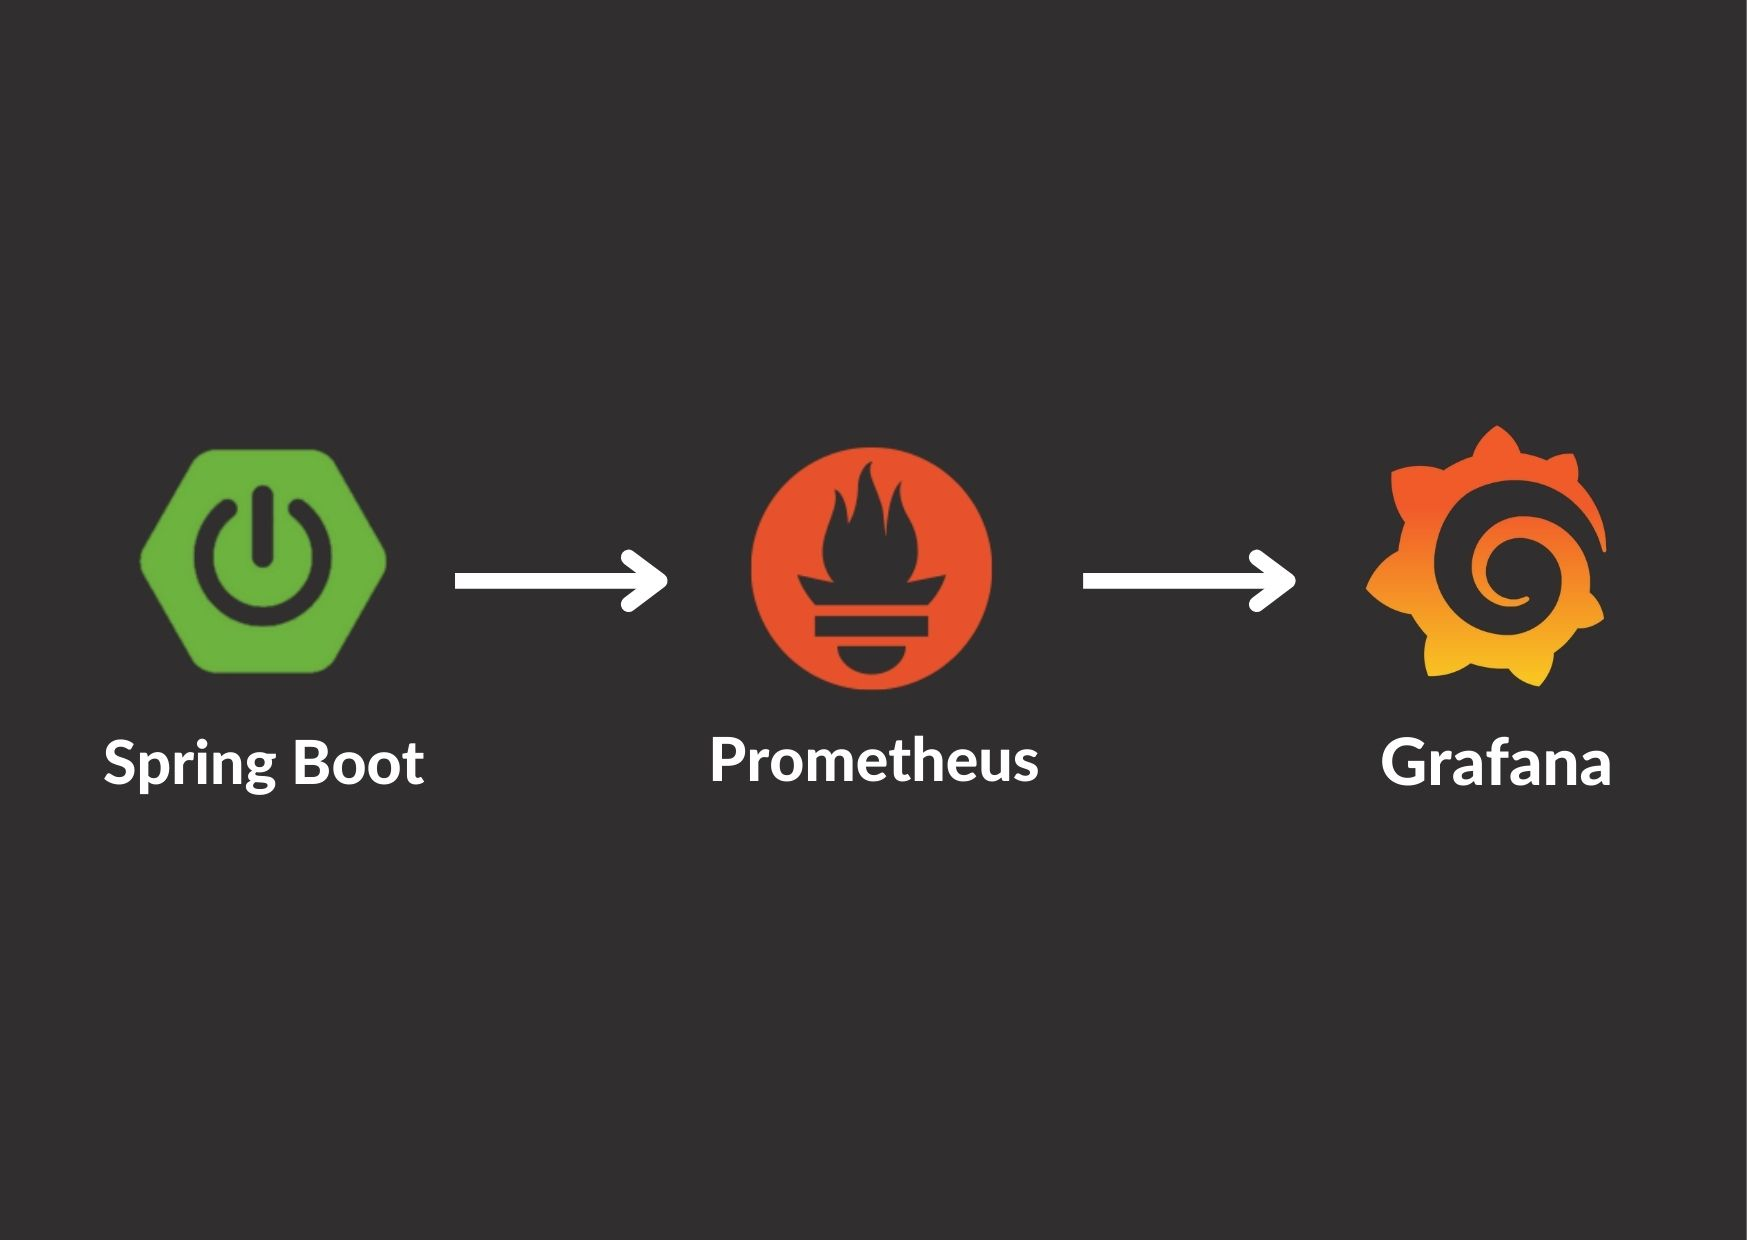
\includegraphics[width=0.5\textwidth]{res/images/cover}
	\caption{Flujo de datos desde la aplicación Spring Boot hasta Grafana. (Fuente~\cite{prometheus-flow}).}
	\label{fig:prometheus-flow}
\end{figure}

\subsect{Grafana (Panel de observabilidad)}{grafana}
Grafana es una solución de código abierto para mostrar las métricas que se recogen de las aplicaciones de una
manera amigable en paneles personalizables~\cite{what-is-grafana}.\ Permite estudiar, analizar y monitorizar
aplicaciones a lo largo del tiempo gracias a las marcas de tiempo proporcionadas junto con los datos que se
recolectan.\ Se puede conectar con muchas fuentes de datos, como Graphite, Prometheus, ElasticSearch, MySQL, etc.\
Una ventaja de Grafana es que ofrece una solución \quoted{on-premise}, que permite desplegar una instancia propia en
el mismo servidor donde se ejecuta la aplicación.\ De esta manera, se garantiza la seguridad y protección de los
datos, ya que no se exponen a Internet de manera directa.

Para la configuración de Grafana en el entorno de producción, se necesita un contenedor Docker que utilice la imagen
\monoFont{grafana/grafana-oss} y exponga un puerto para permitir conexiones (el 4046 en este caso).\ A continuación,
se presenta una configuración básica para ejecutar una instancia de Grafana:

\begin{codeBlock}
	\begin{minted}[
		baselinestretch=1.1,
		fontsize=\footnotesize,
		tabsize=2,
	]{yaml}
version: '3.7'
services:
  grafana:
    image: grafana/grafana-oss:9.3.1
    ports:
      - "4046:3000"  # Mapeo de puertos (HOST:CONTENEDOR)
    volumes:
      - grafana-storage:/var/lib/grafana  # Se define el volumen 'grafana-storage'
    env_file:
      - GF_SECURITY_ADMIN_USER=<usuario>
      - GF_SECURITY_ADMIN_PASSWORD=<contraseña>
    networks:
      - rschat-net  # Se asigna la red interna para comunicarse con otros servicios
	\end{minted}
	\caption{Configuración mínima para ejecutar un contenedor con Grafana.}
	\label{cod:grafana-docker-compose}
\end{codeBlock}

En este proyecto se ha utilizado un panel importado desde las plantillas de la comunidad de Grafana para su utilización
con Spring Boot y Prometheus~\cite{spring-dashboard} al que se le han añadido más paneles (para los logs y otras
métricas).\ Algunos de los tipos de paneles que se pueden añadir son de tipo numérico o texto, gráficas, histogramas,
mapas de calor, tablas, entre otros~\cite{visualizaciones-grafana}.

\begin{figure}[H]
	\centering
	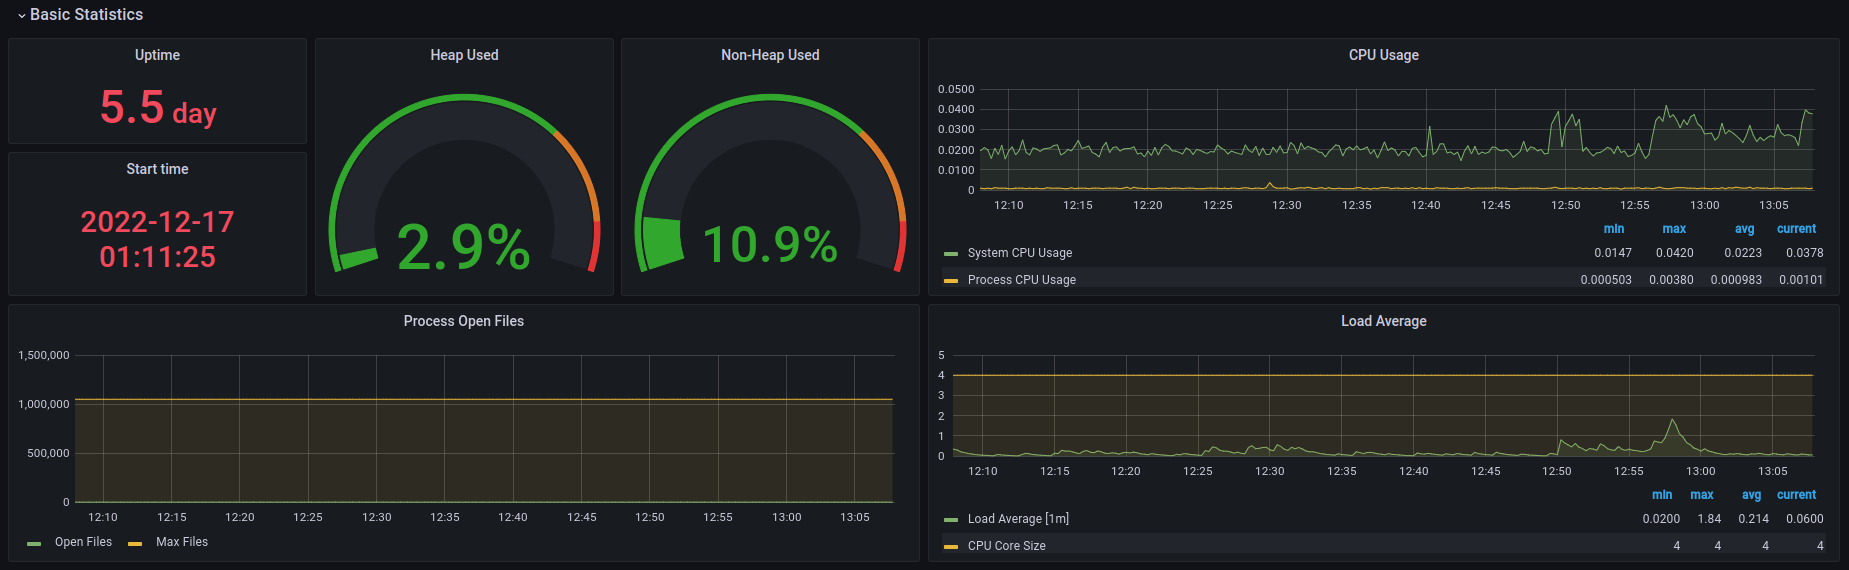
\includegraphics[width=\textwidth]{res/images/GrafanaDashboard_1}
	\caption{Visualización de métricas relacionadas con los recursos del sistema utilizados y tiempo de actividad.}
	\label{fig:grafana-dashboard_1}
\end{figure}

\begin{figure}[H]
	\centering
	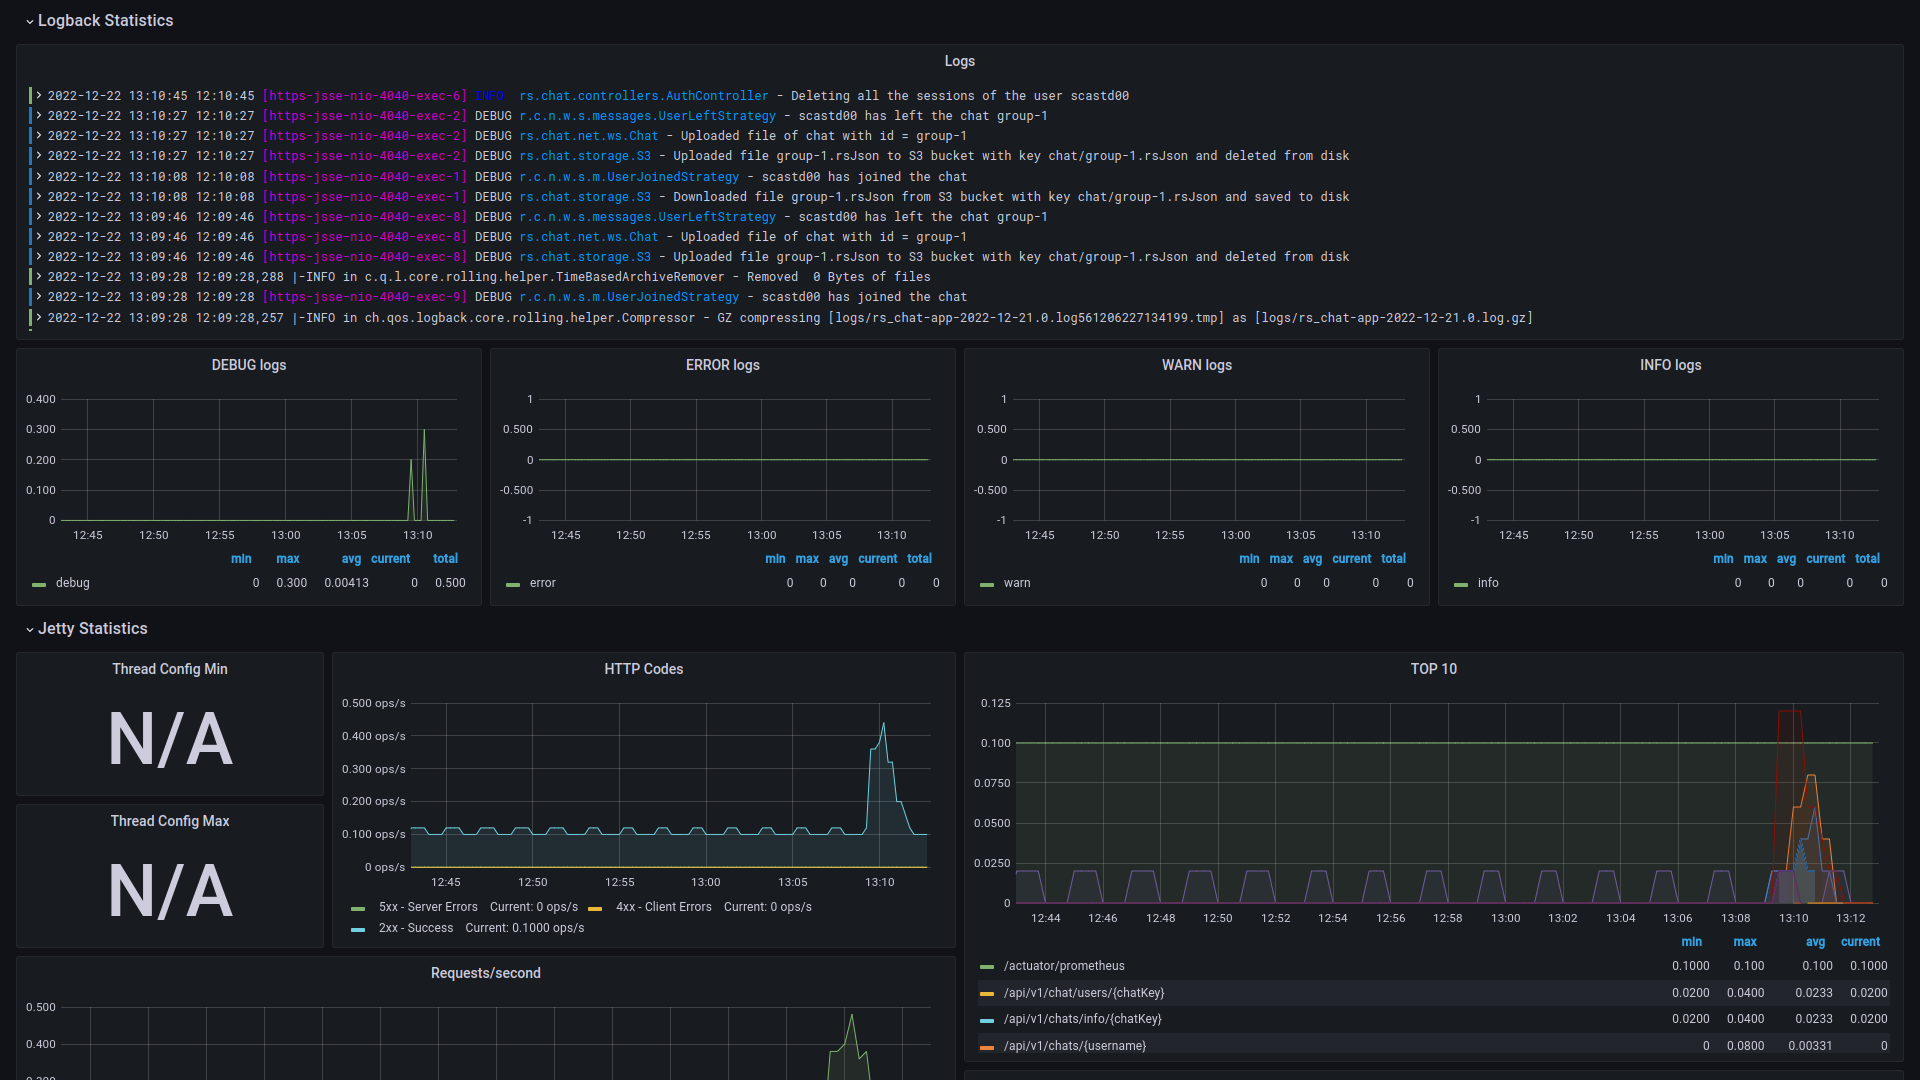
\includegraphics[width=\textwidth]{res/images/GrafanaDashboard_2}
	\caption{Visualización de métricas relacionadas con los logs y peticiones HTTP.}
	\label{fig:grafana-dashboard_2}
\end{figure}

Para que Grafana muestre toda esta información, se deben configurar 2 fuentes de datos de las cuales extraer las
métricas.\ Para establecer estos ajustes, accedemos a \monoFont{Configuration >~ Data Sources} y añadimos un
\quoted{data source} para Prometheus y otro para Loki, con la URL que provee las métricas (el nombre del contenedor con
el puerto interno, ya que se usa la misma red para todos los servicios):

\begin{itemize}
	\item Prometheus: \monoFont{http://prometheus:9090}
	\item Loki: \monoFont{http://loki:3100}
\end{itemize}
\label{itm:grafana-data-sources}

\subsect{Loki (Agregación de logs)}{loki}
Loki es una herramienta de agregación de logs, que permite almacenar, indexar y consultar logs de manera eficiente, ya
que se basa en el uso de etiquetas (para el agrupamiento y filtrado de logs) dejando el mensaje original sin
modificar~\cite{loki-docs}.
Para el funcionamiento de Loki es necesario disponer de un agente que se encargue de enviar los logs a la instancia de
Loki, y en este proyecto se ha utilizado Promtail, explicado en la siguiente subsección.
La configuración necesaria para que Grafana pueda recoger los logs de Loki es sencilla, ya que se añade un fichero
\monoFont{yaml} con la configuración de la fuente de datos de Loki~\cite{loki-config-file} y el servicio en el
fichero \monoFont{docker-compose.yaml}:

\begin{codeBlock}
	\begin{minted}[
		baselinestretch=1.1,
		fontsize=\footnotesize,
		tabsize=2,
	]{yaml}
  loki:
    image: grafana/loki:2.7.0
    container_name: loki
    restart: unless-stopped
    ports:
      - "4045:3100"
    volumes:
      # Habilitar la lectura del fichero de configuración desde el contenedor
      - ./config/loki.yaml:/etc/loki/loki-config.yaml
    command: -config.file=/etc/loki/loki-config.yaml
    depends_on:
      - promtail
    networks:
      - rschat-net
	\end{minted}
	\caption{Servicio de Loki para el registro de logs.}
	\label{cod:loki-docker-compose}
\end{codeBlock}

\subsect{Promtail (Agente de logs)}{promtail}
Promtail es un agente (o cliente) de logs, que los recoge y los convierte en flujos que puede enviar a Loki (ver
imagen~\ref{fig:promtail}) a través de una API HTTP~\cite{loki-docs}.\ La configuración de Docker para Promtail es
similar a la de
Loki, ya que se añade un fichero \monoFont{yaml} con la configuración de la fuente de datos de Promtail y el servicio
en el fichero \monoFont{docker-compose.yaml}:

\begin{codeBlock}
	\begin{minted}[
		baselinestretch=1.1,
		fontsize=\footnotesize,
		tabsize=2,
	]{yaml}
  promtail:
    image: grafana/promtail:2.7.0
    container_name: promtail
    restart: unless-stopped
    ports:
      - "4044:9080"
    volumes:
      - /var/log:/var/log
      # Habilitar la lectura del fichero de configuración desde el contenedor
      - ./config/promtail.yaml:/etc/promtail/promtail.yaml
      # Habilitar acceso a los logs de los contenedores
      - /var/lib/docker/containers:/var/lib/docker/containers
    command: -config.file=/etc/promtail/promtail.yaml
    depends_on:
      - rschat
    networks:
      - rschat-net
	\end{minted}
	\caption{Servicio de Promtail para la recolección de logs.}
	\label{cod:promtail-docker-compose}
\end{codeBlock}

\begin{figure}[ht]
	\centering
	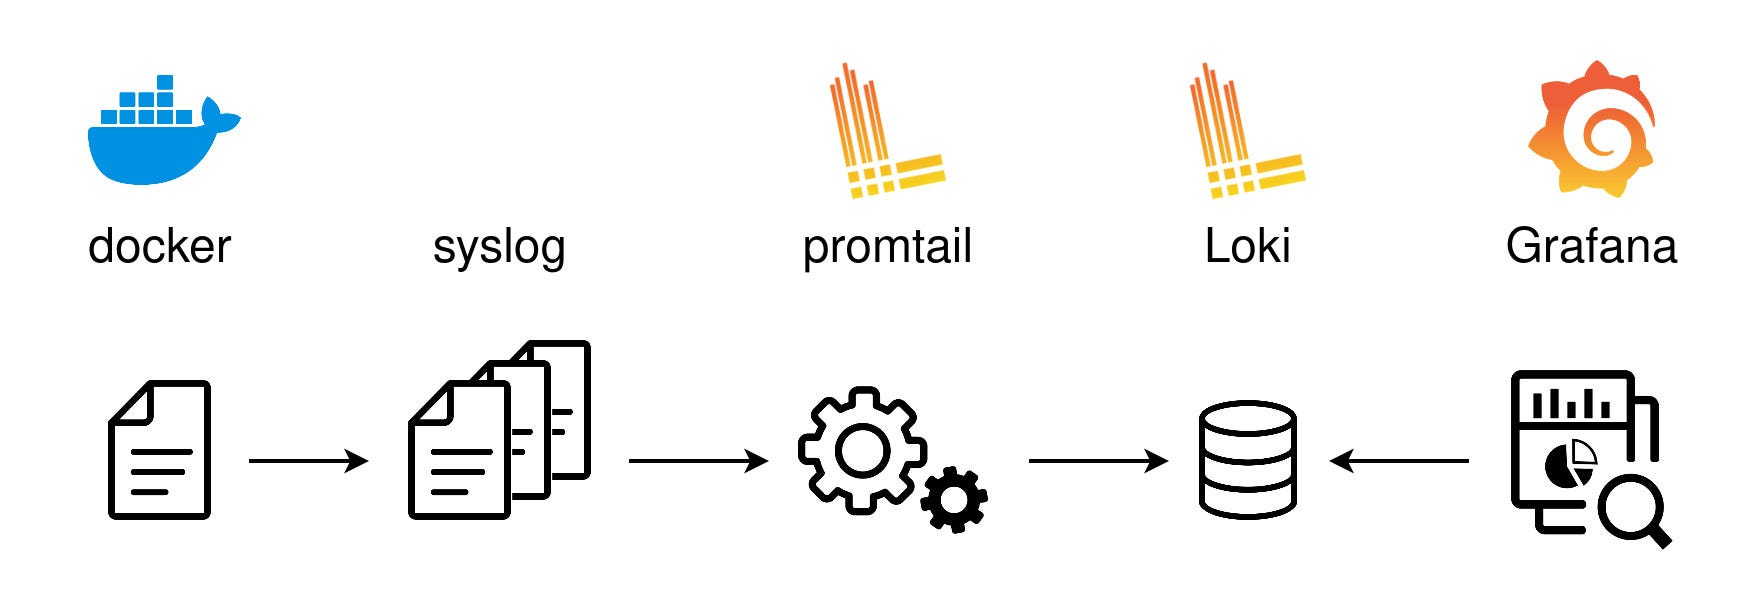
\includegraphics[width=0.8\textwidth]{res/images/loki-promtail-architecture}
	\caption{Flujo de logs entre Promtail y Loki.}
	\label{fig:promtail}
\end{figure}

El formato de las trazas que exporta Promtail se ha ajustado para que se permita la visualización tanto por fichero,
como por el nombre del contenedor que genera el log.\ Para ello, el fichero \monoFont{promtail.yaml}
contiene una sección \monoFont{pipeline\_stages}, con la configuración de los \quoted{stages} que se aplican a las
trazas antes de enviarlas a Loki.\ La más importante es la que se encarga de añadir las etiquetas
\monoFont{container\_name}, usando una expresión regular que extrae el nombre del contenedor a partir de una etiqueta
asociada a cada traza:

\begin{codeBlock}
	\begin{minted}[
		baselinestretch=1.1,
		fontsize=\footnotesize,
		tabsize=2,
	]{yaml}
    pipeline_stages:
      # ...
      - regex:  # Nombre del contenedor en el valor de "tag"
          expression: (?P<container_name>(?:[^|]*[^|]))
          source: tag
      # ...
	\end{minted}
	\caption{Stage para obtener el nombre del contenedor con una expresión regular a partir de la etiqueta
	\monoFont{tag}.}
	\label{cod:promtail-regexp-container-name}
\end{codeBlock}

\subsect{NSFWPY}{nsfwpy}
NSFWPY es un detector de contenido no seguro para el trabajo (NSFW, por sus siglas en inglés), que se ha utilizado para
detectar imágenes inapropiadas en los mensajes de los usuarios.\ Es un programa escrito en Python, que consiste en
un pequeño servidor HTTP (utilizando Flask) que recibe una imagen en formato \monoFont{base64} y devuelve un JSON con
la predicción de la imagen.\ Para realizar la predicción, se utiliza el modelo de inteligencia artificial
\href{https://github.com/GantMan/nsfw_model}{\textit{GantMan/nsfw\_model}}~\cite{nsfw-model-repo},
que está pre-entrenado con imágenes de contenido NSFW y SFW (seguro para el trabajo).\ El modelo devuelve una
predicción de la clase a la que pertenece la imagen, con una probabilidad entre 0 y 1, siendo 0 la probabilidad de
que la imagen sea SFW y 1 la probabilidad de que la imagen sea NSFW\@.\ El modelo está entrenado para detectar 5
clases de imágenes NSFW:
\begin{itemize}
	\item Drawings (Dibujos): Imágenes de dibujos animados o hechos a mano.
	\item Hentai (Manga): Imágenes de manga o anime con contenido sexual.
	\item Neutral: Imágenes neutrales.
	\item Porn (Pornografía): Imágenes que tiene contenido pornográfico.
	\item Sexy (Sensual): Imágenes que tienen un tono sensual.
\end{itemize}

Para que la aplicación pueda utilizar el detector NSFWPY, se ha creado un nuevo servicio en el fichero
\monoFont{docker-compose.yaml}, que se encarga de ejecutar el programa de Python con el detector, y se ha añadido
una nueva ruta en la API de RSChat, que se encarga de llamar al detector NSFWPY\@.

\begin{codeBlock}
	\begin{minted}[
		baselinestretch=1.1,
		fontsize=\footnotesize,
		tabsize=2,
	]{yaml}
  nsfwpy:
    image: nsfwpy:latest
    container_name: nsfwpy
    ports:
      - "4042:4042"
    networks:
      - rschat-net
    healthcheck:
      test: curl -f http://localhost:4042/api/v1/health -s > /dev/null || exit 1
      interval: 2m
      timeout: 10s
      retries: 3
	\end{minted}
	\caption{Servicio de NSFWPY para la detección de imágenes NSFW.}
	\label{cod:nsfw-docker-compose}
\end{codeBlock}

Este modelo se ha conocido a través a la página web \href{https://nsfwjs.com/}{NSFWJS}~\cite{nsfwjs}, que lo utiliza
para el análisis de las imágenes desde el propio navegador del usuario, sin necesidad de enviarlas a un servidor.
La web permite probar el modelo con imágenes que se pueden arrastrar y soltar en la página, y muestra la
predicción del modelo para cada una de ellas.\ Las figuras~\ref{fig:nsfwjs-drawing} y~\ref{fig:nsfwjs-porn} muestran
dos ejemplos de predicción del modelo para dos imágenes diferentes.

\begin{figure}[H]
	\centering
	\begin{minipage}[c]{0.46\linewidth}
		\centering
		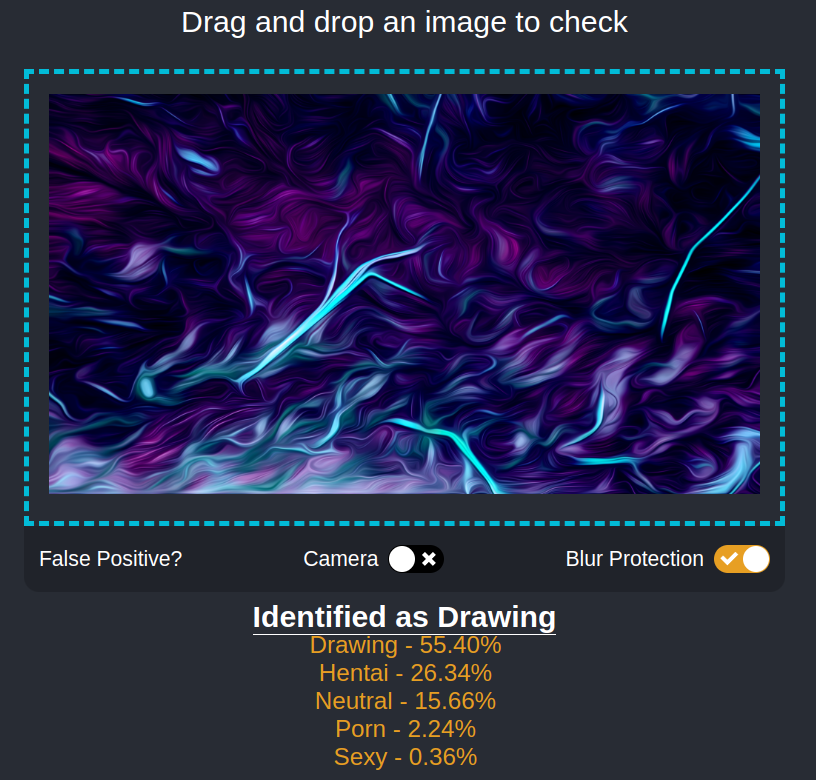
\includegraphics[width=\textwidth]{nsfwjs-drawing}
		\caption{Predicción para una\\ imagen de fondo de pantalla.}
		\label{fig:nsfwjs-drawing}
	\end{minipage}
	\hfill
	\begin{minipage}[c]{0.46\linewidth}
		\centering
		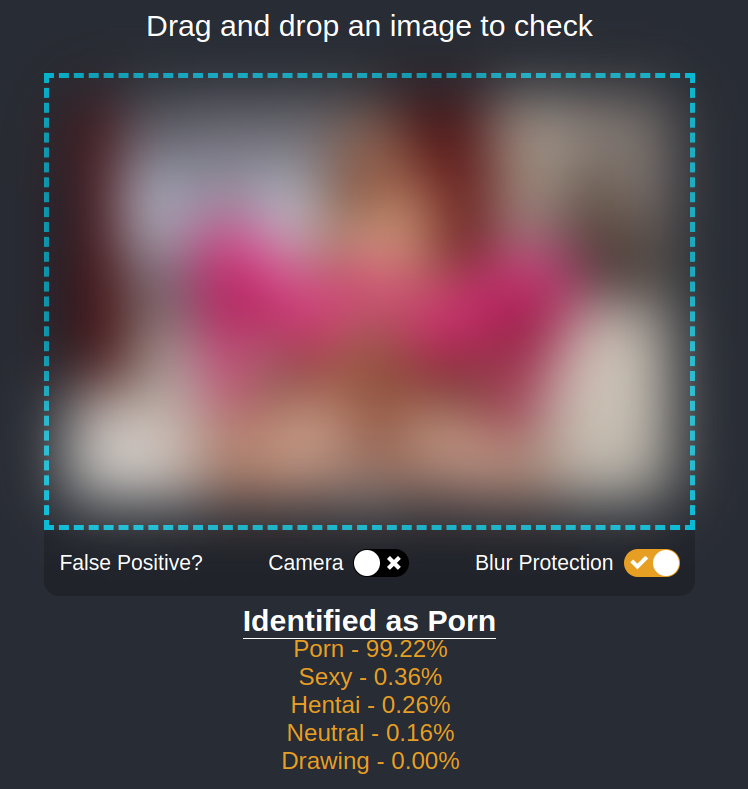
\includegraphics[width=\textwidth]{nsfwjs-porn}
		\caption{Predicción para una\\ imagen pornográfica.}
		\label{fig:nsfwjs-porn}
	\end{minipage}
	\label{fig:nsfwjs-example}
\end{figure}

Como se puede observar en las imágenes, la web muestra la predicción del modelo para cada una de las clases como
un porcentaje.\ En el caso de la imagen de la izquierda, se puede ver que el modelo ha predicho que la imagen es
un dibujo con un 55.40\% de probabilidad, mientras que en la imagen de la derecha, el modelo ha predicho que
la imagen es pornográfica con un 99.22\% de probabilidad.
